\documentclass[Main.tex]{subfiles}
\begin{document}
\section{Experimenten}
Voor het verder verklaren van de experimenten zijn er een aantal zaken die vermeld moeten worden. De volgorde waarin de experimenen zijn uitgevoerd is van belang. Bij de meeste experimenten wordt er gebaseerd op de resultaten van de voorgaande experimenten. Er zijn verschillende beoordelingswijzen die gebruikt worden bij het onderzoeken van de experimenten. Enerzijds testen de experimenten op oplossingsgraad\footnotemark[\ref{note:oplossingsgraad}] en anderzijds op de tijdsmarge die het algoritme nodig heeft. 
\par
Indien er niet gebaseerd wordt op de resultaten van vorige experimenten, dan zijn sommige van de latere experimenten enorm tijdrovend. Deze tijdrovende experimenten tonen ook niets aan wat niet aangetoond kan worden met de huidige manier van experimenteren.
\par
Alle experimenten zijn uitgevoerd op een \textit{2.26 GHz Intel Core 2 Duo} processor. Het aantal iteraties van elk experiment is 500 en de gebruikte diepte van de boom is tot en met 5 termen breed, een voorbeeld van een vergelijking op die diepte is $K1^{K2}+K3 \div K4*K5$. Bij elk van deze iteratie worden er twee voorbeelden gegeven waaraan de vergelijking moet voldoen.

\subsection{Oude pruning}

In de opvoorhand gegenereerde boom bestaat er de mogelijkheid om te prunen. Op experimentele wijze wordt nu onderzocht hoeveel knopen overbodig zijn in de bewerkingsboom. Hiervoor wordt er een vergelijking gemaakt tussen het aantal knopen van de originele boom en het aantal knopen is deze nieuwe boom.
\par Zoals op de figuur te zien valt is er een stagnatie vanaf diepte 5 waarbij er 35\% minder knopen aanwezig zijn ten opzichte van de originele boom. Dit heeft een enorme invloed op het aantal mogelijkheden die moeten afgegaan worden bij het evalueren van alle knopen.
\begin{center}
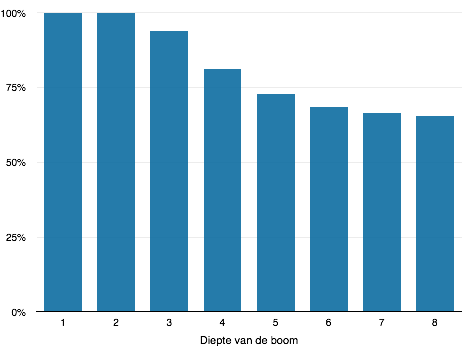
\includegraphics[width=\columnwidth]{treePrune.png}
\end{center}

\subsection{Gewichten}
De volgende stap is het bepalen welke invloed het toevoegen van een set van constante waarden heeft op de snelheid en de oplossingsgraad van het algoritme. In dit experiment worden er vier verschillende sets van waarden gebruikt, deze zijn $(1,2,3), (1,2,3,4,5), (1,2,3,5,7)$ en $(1,2,3,4,5,6,7,8,9)$. Om goed te kunnen vergelijken wordt er op de grafiek de benodigde tijd getoond zonder constanten. Hierdoor kan men bepalen welke invloed het toevoegen van constanten heeft op de snelheid van het algoritme.

\begin{center}
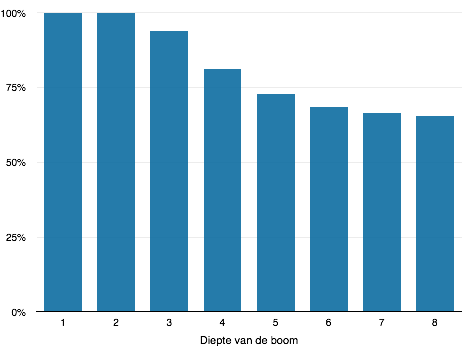
\includegraphics[width=\columnwidth]{treePrune.png} %TODO Tijden vergelijken
\end{center}

Uit de looptijd van de verschillende sets van waarden valt af te leiden dat deze stijgt naar mate er meer waarden worden toegevoegd. Deze stijging was verwacht. Om de voorkeur te laten uitgaan naar meer constanten is het dus nodig dat de oplossingsgraad stijgt bij het toevoegen van deze constanten. 

\begin{center}
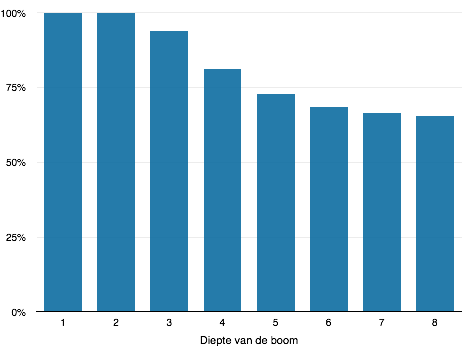
\includegraphics[width=\columnwidth]{treePrune.png} 
\end{center}

Door toevoeging van meer constanten wordt er vaker een passende vergelijking gevonden. Indien de vergelijking gemaakt wordt tussen de verschillende sets van constanten, dan valt meteen op dat de oplossingsgraad stijgt volgens een andere curve dan het tijdsverloop. Om nu het algoritme te verbeteren wordt er een afweging gemaakt worden tussen tijd en oplossingsgraad. Uit deze afweging wordt er een set van getallen gekozen die het meest geschikt lijken voor het gegeven probleem. In dit geval is de set van \textit{(1,2,3,5,7)} gevonden als meest geschikte set van constante waarden. 

\subsection{Prunen op vergelijkingen}

Bij de verschillende aanpakken ontstaan er verschillende bomen. De manier waarop deze bomen geoptimaliseerd kunnen worden is dus ook verschillend. De ene is afhankelijk van de productieregels van de contextvrije grammatica en andere is ook afhankelijk van de productieregels maar ook van de gegevens waarmee het algoritme moet werken. 
\par 
Mogelijke voorbeelden van het verschil in pruning ligt op het vlak dat er meer optimalisaties kunnen gebeuren. Verdere optimalisaties zijn bijvoorbeeld het weglaten van knopen waarbij men $1$ of $0$ bekomt door middel van respecitievelijk $K1-K1$ en $K1/K1$. Maar ook enkel knopen toe te laten waarbij $K1$ groter is dan $K2$ in gevallen zoals $K1+K2$ of $K1*K2$ aangezien er door de volgorde van bewerkingen geen verschil bestaat tussen bijvoorbeeld $K1*K2$ en $K2*K1$.
\par 

Het verschil in verminderen van het aantal knopen is significant genoeg om het tijdsverlies met het opstellen van de boom bij elke dataset te compenseren. Vanwege deze reden is de keuze voor verder onderzoek op de methode gevallen waarbij de boom op 'runtime' wordt opgesteld. 

\subsection{Brute force vs Optimaliseren}

Als laatste experiment is het nu interessant om te zien wat het verschil in tijd en oplossingsgraad is van het uiteindelijke algoritme ten opzichte van de originele brute-force manier. Bij dit experiment word er gebruik gemaakt van alle optimalisaties die hierboven beschreven staan.

\begin{center}
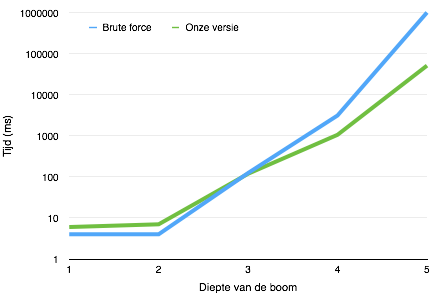
\includegraphics[width=\columnwidth]{bruteVSOpt.png}
\end{center}

\end{document}